\documentclass[a4paper, 11pt, twocolumn]{article}
\usepackage[utf8]{inputenc}
\usepackage[left=2cm, top=2cm, text={17cm, 25cm}]{geometry}
\usepackage{times}
\usepackage{graphicx}
\usepackage[unicode, colorlinks, hypertexnames=false, citecolor=red]{hyperref}


\begin{document}
	%%%%%%%%%%%%%%%%%%%%%%%%%%%%%%%% Title page %%%%%%%%%%%%%%%%%%%%%%%%%%%%%%%%
	\twocolumn[
		\begin{@twocolumnfalse}
			\begin{center}
				{\Large
					Brno University of Technology \\
					Faculty of Information Technology \\
				}
				{
\includegraphics[width=0.4 \linewidth]{logo.pdf}} \\

				{\LARGE
					Microprocessors and Embedded Systems \\
					Project\,--\,Bluetooth metronome \\[0.4cm]
				}

				{\large
					Krištof Teplan (xtepla01) \\
					\texttt{xtepla01@stud.fit.vutbr.cz} \\
					\today
				}
			\end{center}
		\end{@twocolumnfalse}
	]
	%%%%%%%%%%%%%%%%%%%%%%%%%%%%%%%% Abstract %%%%%%%%%%%%%%%%%%%%%%%%%%%%%%%%
	\section{Abstract}

	The goal of the project is to create a device with a buzzer that will create a metronome for musicians
     with the help of the ESP-WROOM-32 microcontroller on the Wemos D1 R32 board. The device works
     autonomously in preset values. The user can connect to the device using
     web-bluetooth and change these preset values. The device remembers these
     values unless we restart it or disconnect it from the power supply. current. User can set
     these 3 integer values for buzzer: beeps per minute(1-255), volume(0-8), beep length (1-255ms).
    



	%%%%%%%%%%%%%%%%%%%%%%%%%%%%%%%% Circuit setup %%%%%%%%%%%%%%%%%%%%%%%%%%%%%%%%
	\section{Circuit setup}

	
    \begin{figure}[ht]
		\centering
		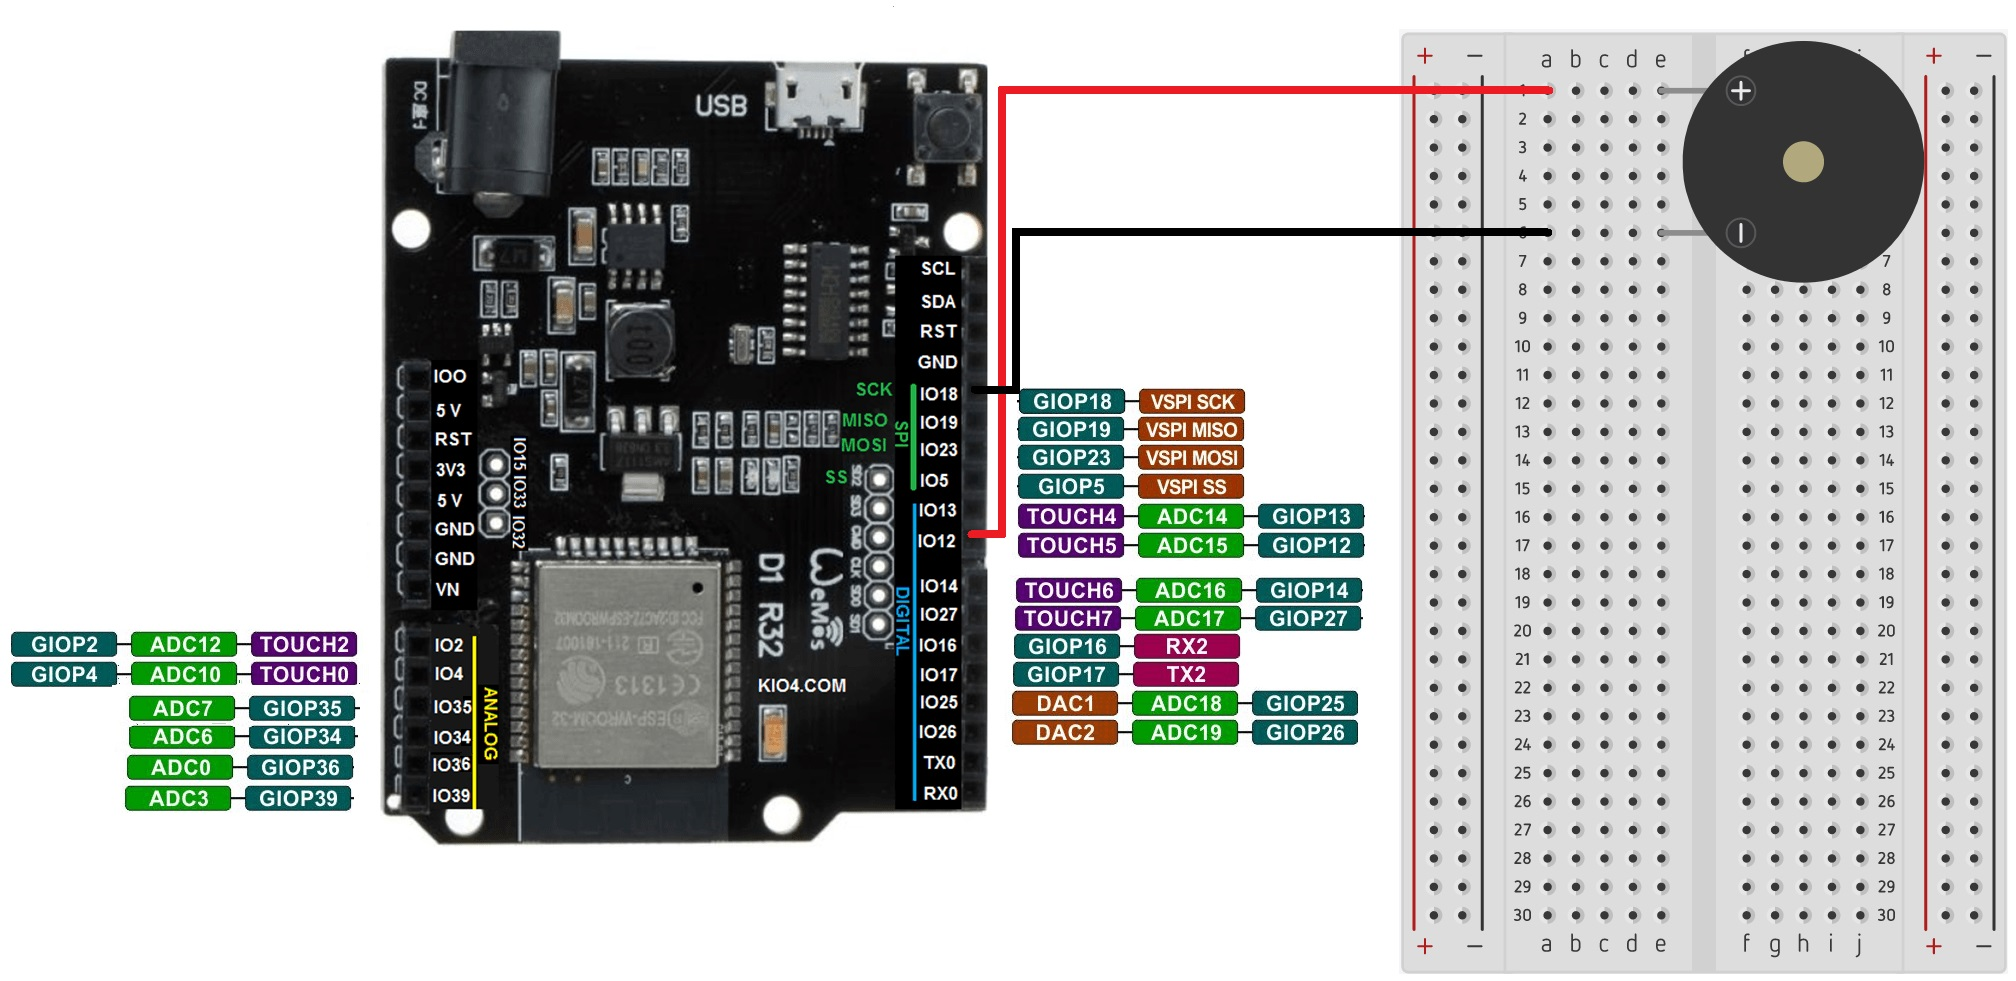
\includegraphics[width=0.8 \linewidth]{circuit_schema.jpg}

		\caption{The buzzer is connected with the cathode to the GPIO~12 port and the anode to GND}
		\label{fig:circuit}
	\end{figure}
	%%%%%%%%%%%%%%%%%%%%%%%%%%%%%%%% Implementation %%%%%%%%%%%%%%%%%%%%%%%%%%%%%%%%
	\section{Implementation}
    	The code implementation for the microcontroller is in the file \texttt{src/main.c}. Code implementation
        the webpage is in the file webpage\textunderscore bluetooth.html.

	\subsection{Implementation of the program for microcontroler: main.c}
        It implements the behavior of esp-32 and its peripherals using libraries \texttt{ArduinoBLE.h}, 
        \texttt{Ticker.h} and \texttt{math.h}. The core of the implementation is the BLE(Bluetooth low energy) setup,
         its service and characteristics, two timers, communication of 3 key values and their processing.
    
    \subsubsection{Globál frame}
        Initializes the UUID (Universally unique identifier) for the local service and its characteristics,
         default values \texttt{BPM}, \texttt{volume} and \texttt{beepLength}, pointers to two timers.
         It further defines the interrupt handlers invoked by these timers. Interrupt handling from timer
         \texttt{timerTurnON}: \texttt{void IRAM\_ATTR beep\_ON\_interrupt} turns on the beep sound by changing
         voltage on the cathode of the buzzer using PWM(Pulse Width Modulation - simulates analog output) in values 
         0-255 converted from volume(0-8) values exponentially. Finally, it resets and starts the second timer 
         \texttt{timerTurnOFF}. Interrupt handling from timer \texttt{timerTurnOFF}: \texttt{void IRAM\_ATTR 
         beep\_OFF\_interrupt} turns off the buzzer beep and starts the timer \texttt{timerTurnON}.

    \subsubsection{void setup()}
        Sets buzzer pin and red LED(blinking LED is synchronized with buzzer) pin to \texttt{OUTPUT} mode. Initializes timers into prepared pointers,
        assigns them interrupt handling functions, how much they should count to (calculated from \texttt{beepLength} and \texttt{BPM}),
        until the interrupt is triggered and the divider to 80. At an APB(Advanced periferial bus) speed of 80Mhz, divider 80 guarantees that the timers
        add up every millionth of a second. The \texttt{timerTurnOFF} timer starts, which starts the mutual loop
        starting both timers. The BLE functionality will start. The name under which the esp-32 is displayed(\texttt{ESP32-BT metronome}) on bluetooth is set.
        The service will begin to be promoted with characteristics added to it.

    \subsubsection{void loop()}
        It is waiting for the central unit to be connected via bluetooth. When the central office is connected, it checks in an endless loop whether
        were the characteristics of the bluetooth service overwritten, if so it saves these values in variables \texttt{BPM}, \texttt{volume} and 
        \texttt{beepLength}. According to these values, the timing of timers is and buzzer volume is adjusted.
        
    \begin{figure}[ht]
        \centering
        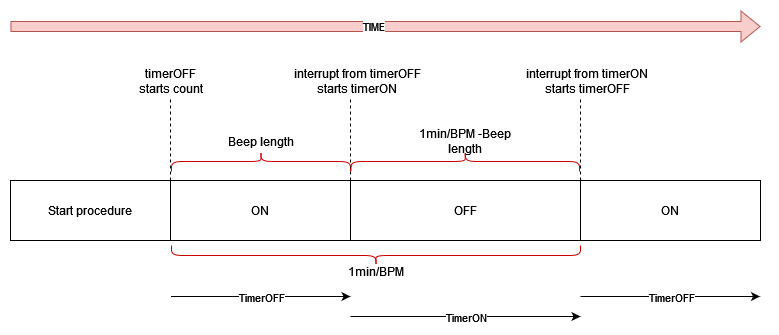
\includegraphics[width=1 \linewidth]{diagram_in_time.jpg}

        \caption{Diagram of interrupt timing}
        \label{fig:timediagram}
    \end{figure}

    \subsection{Implementation of a website using webbluetooth: webpage\textunderscore bluetooth.html}
    \begin{figure}[ht]
		\centering
		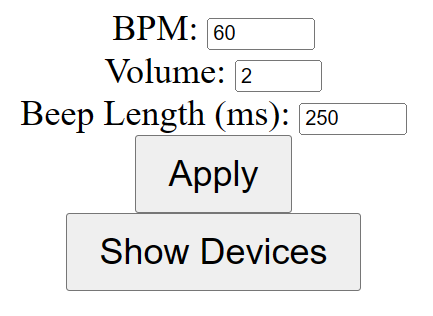
\includegraphics[width=0.8 \linewidth]{webpage_screen.png}

		\caption{Website user interface}
		\label{fig:webpage}
	\end{figure}
 
    The page shows the user 3 text fields for 3 metronome settings. Buttons for connection via BLE
    and a button to apply the selected settings. The corresponding default values are displayed in the input fields corresponding
    with basic microcontroller setup. The value of the characteristics is sent in 8-bit form and the volume has 9 levels, that's why they are
    retricted as follows: BPM(1-255), Volume(0-8), Beep Length(1-255). The values must also satisfy the equation:
    \[\frac{60000}{bpm} > beepLength\] Otherwise, the beep would be as long as or longer than the full period of
    metronome, so the individual beeps would not be separated from each other. The values are not applied unless we are connected to the microcontroller.
    Violation of restrictions by the user or system failure is always indicated by an error message or warning in the text field under
    control elements. While searching for devices, filter is applied so only device with right name and our custom service will appear to user.

    %%%%%%%%%%%%%%%%%%%%%%%%%%%%%%%% Findings %%%%%%%%%%%%%%%%%%%%%%%%%%%%%%%%
	\section{Findings}
    I observed a strange behavior of the buzzer. Despite the fact that it has its own oscillator, it changes its tone when the simulated voltage of the PWD is lower. I would explain this by saying that the buzzer does not have enough power and some of the vibrations are lost. Another interesting finding is
    that the frequency of the internal timers of the microcontroller is tied to the frequency of the APB (Advanced peripheral bus) which is 80Mhz and not to the frequency
    of core. I explain it by the fact that the peripherals cannot be controlled by the variable frequency of the core, which is at most 240Mhz. Timer divider
    is stored as a 16-bit value, so milliseconds could not be calculated directly because $80Mhz/80000 = 1 millisecond$ and $80000>65535$ so I
    had to use a larger bit width of the timer counter (64-bit).

    %%%%%%%%%%%%%%%%%%%%%%%%%%%%%%%% Conclusion %%%%%%%%%%%%%%%%%%%%%%%%%%%%%%%%
    \section{Conclusion}
    The project solution implements all the functionality requirements. In addition, I added the ability to adjust the length of the beep, a large amount of error detection and warnings/reports for the user. For practical reasons, I also added a blinking LED, which is synchronized with the buzzer. The topic itself is very interesting and practical, despite the fact that I found it more challenging writing website code as the controller code itself.
    
\end{document}